\chapter{Proposta}
\label{ch:proposta}

A proposta principal deste trabalho é desenvolver uma versão do algoritmo FSS aplicando em problemas dinâmicos com domínio contínuo. Serão aplicados as técnicas de manutenção da diversidade populacional estudadas neste trabalho, para avaliar a influência de cada uma em cada aspecto do algoritmo, como desempenho, robustez e satisfabilidade. O algoritmo final terá a possibilidade de alternar nos operadores evolutivos, de modo que cada operador possa ser analisado individualmente (aplicado no FSS) ou em conjunto com outro operador e/ou técnica de manutenção de diversidade populacional.

Com este algoritmo será possível realizar experimentos para validar a relevância dos operadores utilizados para cada classe de problemas, como problemas com dinamismos na função objetivo, no limite das variáveis ou até problemas com restrições dinâmicas. Além disso será possível analisar a interação dos operadores entre si e entre as técnicas de manutenção da diversidade populacional.

Para a realização dos testes serão aplicadas as mesmas métricas de desempenho, satisfabilidade, robustez e diversidade para realizar uma comparação justa e detalhada dos componentes usados no algoritmo final. Com o intuito de melhor entender os componentes e o comportamento do algoritmo FSS, este foi implementado na sua versão canônica estacionária e um estudo de caso é detalhado a seguir na Seção \ref{sec:test_case}.

\section{Estudo de Caso}
\label{sec:test_case}

O algoritmo foi aplicado nas seguintes funções de \textit{benchmarks} estáticas para ter um melhor entendimento do algoritmo estudado: Rosembrock, Rastrigin, Griewank, Ackley e Schefel 1.2 que são descritas na Tabela \ref{tb:benchmarcks}.

\begin{table}[]
\label{tb:benchmarcks}
\centering
\caption{Funções \textit{benchmark}}
\label{my-label}
\newcommand{\specialcell}[2][c]{%
	  \begin{tabular}[#1]{@{}c@{}}#2\end{tabular}}
\begin{tabular}{|c|c|}
\hline
Equações & Representação do espaço \\ \hline
$F_{Rosembrock}(x) = \sum_{i=1}^{n-1} \left[ 100 (x_{i+1} - x_i^2)^2 + (1 - x_i)^2\right]$ & \raisebox{-.5\height}{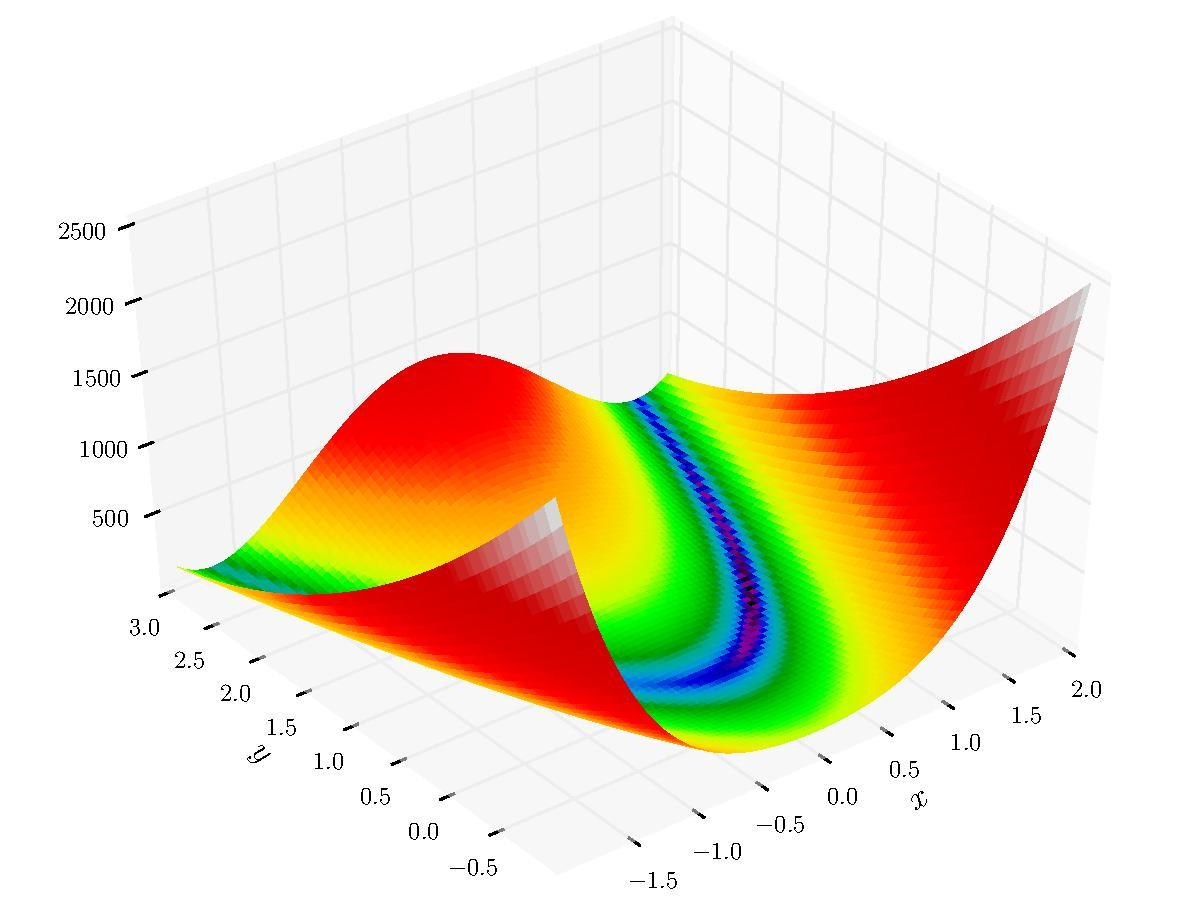
\includegraphics[scale=0.28]{images/f_rosembrock.jpg}} \\ \hline
$F_{Rastrigin}(x) = 10 n + \sum_{i=1}^{n} \left[ x_i^2 - 10\cos(2\pi x_i)\right]$ & \raisebox{-.5\height}{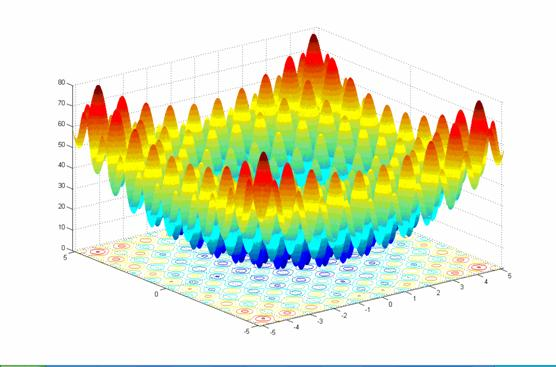
\includegraphics[scale=0.4]{images/f_rastrigin.jpg}} \\ \hline
$F_{Griewank}(x) = 1+ \sum_{i=1}^{n} \frac{x_i^2}{4000} - \prod_{i=1}^{n} \cos$ & \raisebox{-.5\height}{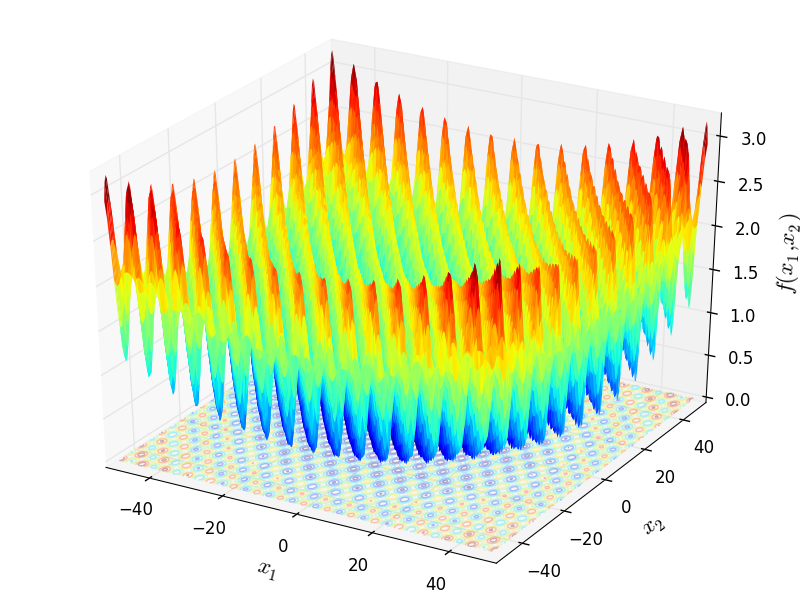
\includegraphics[scale=0.28]{images/f_griewank.png}} \\ \hline
\specialcell{$F_{Ackley}(x) = -20 \exp \left(-0.2 \sqrt{\frac{1}{n} \sum_{i=0}^{n} x_i^2 }\right)$\\$ - \exp \left(\frac{1}{d} \sum_{i=1}^{d} \cos(cx_i) \right) + a + \exp(1)$ }& \raisebox{-.5\height}{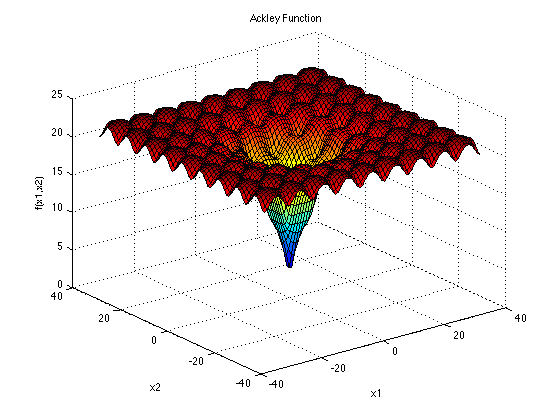
\includegraphics[scale=0.28]{images/f_ackley.png}} \\ \hline
$F_{Schefel 1.2}(x) = \sum_{i=0}^{n} \left(\sum_{j=0}^{i} x_i\right)^2$ & \raisebox{-.5\height}{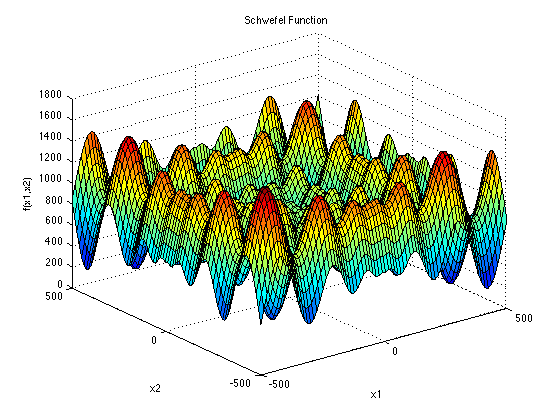
\includegraphics[scale=0.28]{images/f_schafel.png}} \\ \hline
\end{tabular}
\end{table}

Nos testes foram feitas 10 aplicações para cada função, utilizando: 30 dimensões, 30 peixes e 5.000 iterações, sendo que o número total de avaliações de \textit{fitness} é de 300.000. Os parâmetros do FSS foram: o $step_{ind}$ inicial de 0,01 e o final de 0,00001, o $step_{vol}$ inicial de 0,01 e final de 0,0001 e o peso inicial de 2500, variando de 1 a 5000. Os resultados obtidos são apresentados na Tabela \ref{tb:results}

Como pode-se observar nos resultados o FSS tem um bom desempenho para otimização de problemas estáticos e possui uma convergência rápida. Porém a diversidade do sistema é perdida muito rapidamente, fazendo com que a população se torne parecida rapidamente. 

O resultado de performance mais interessantes é o da função de Ackley, em que a otimização ocorre ao longo de todo o processo evolutivo, ao contrário das outras que convergem muito cedo e tem poucas alterações durante o processo evolutivo. Em relação a diversidade, pode-se notar uma perda muito rápida em todas a funções, porém na função de Griewank é observado um curva de perda.

\begin{table}[]
	\centering
	\caption{Tabela de resultados do FSS canônico}\label{tb:results}
	\newcommand{\specialcell}[2][c]{%
	  \begin{tabular}[#1]{@{}c@{}}#2\end{tabular}}
	\begin{tabular}{|c|c|c|c|}
		\hline
		\multicolumn{1}{|l|}{Problemas} & \multicolumn{1}{l|}{Resultado} & \multicolumn{1}{l|}{Performance} & \multicolumn{1}{l|}{Diversidade}\\ \hline
		Rosembrock & \specialcell{24,6284\\(1,68322)} & \raisebox{-.5\height}{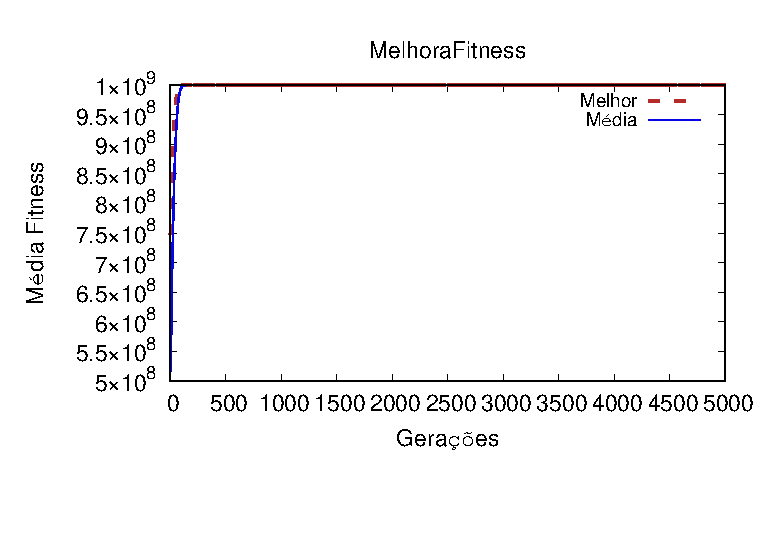
\includegraphics[scale=0.4]{images/p_rosem}} & \raisebox{-.5\height}{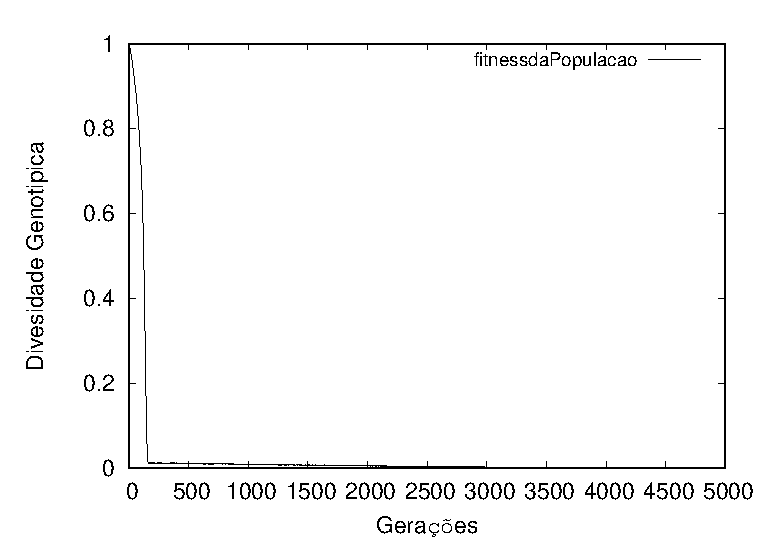
\includegraphics[scale=0.4]{images/d_rosem}} \\ \hline
		Rastrigin  & \specialcell{13,83\\(3,70652)} & \raisebox{-.5\height}{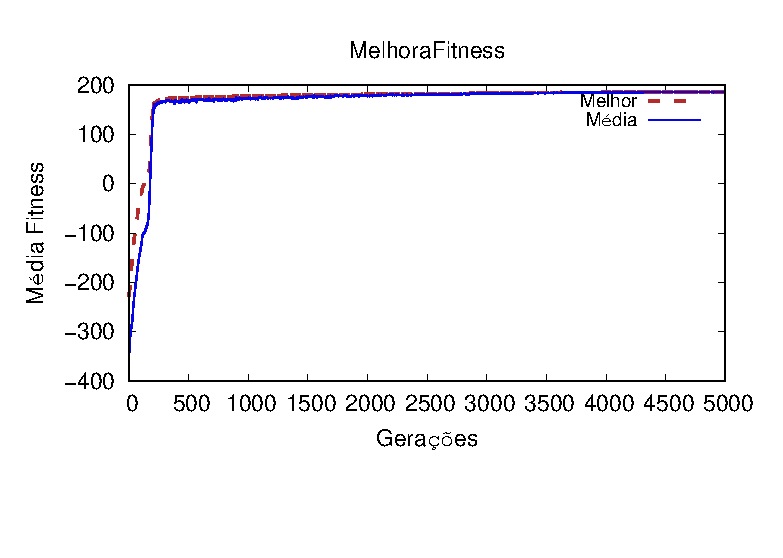
\includegraphics[scale=0.4]{images/p_rast}} & \raisebox{-.5\height}{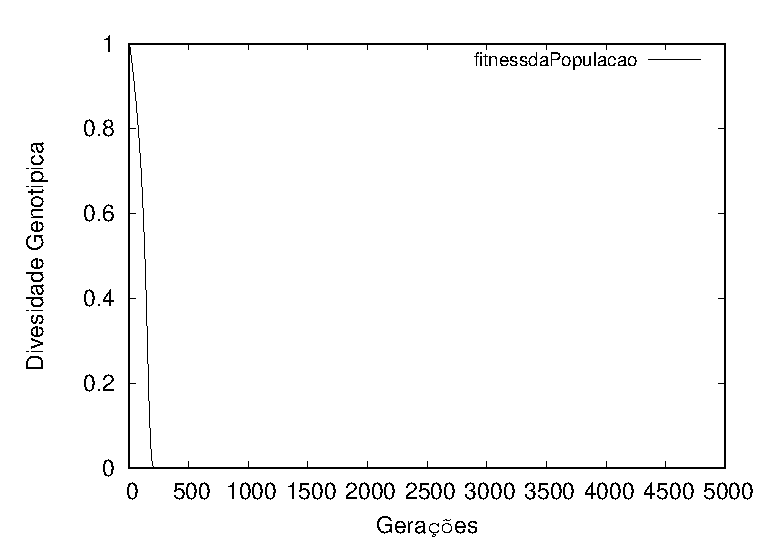
\includegraphics[scale=0.4]{images/d_rast}} \\ \hline
		Griewank  & \specialcell{0,008503\\(0,008108)} & \raisebox{-.5\height}{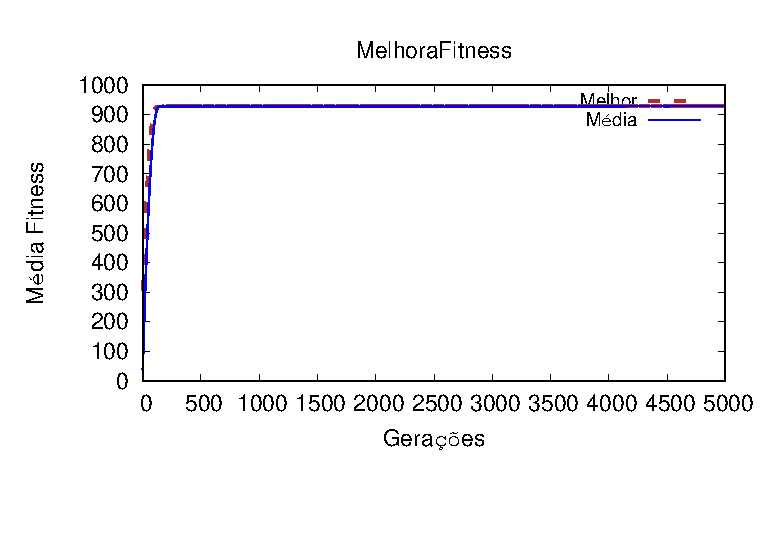
\includegraphics[scale=0.4]{images/p_griew}} & \raisebox{-.5\height}{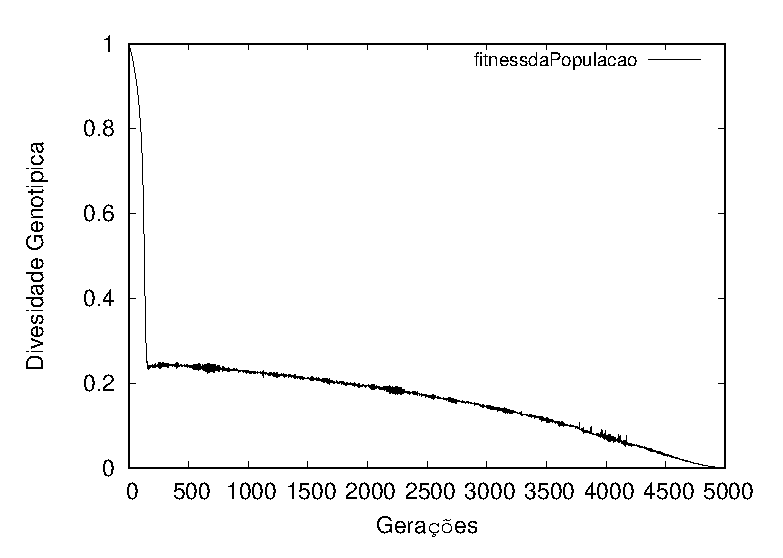
\includegraphics[scale=0.4]{images/d_griew}} \\ \hline
		Ackley  & \specialcell{0,003412\\(0,000491)} & \raisebox{-.5\height}{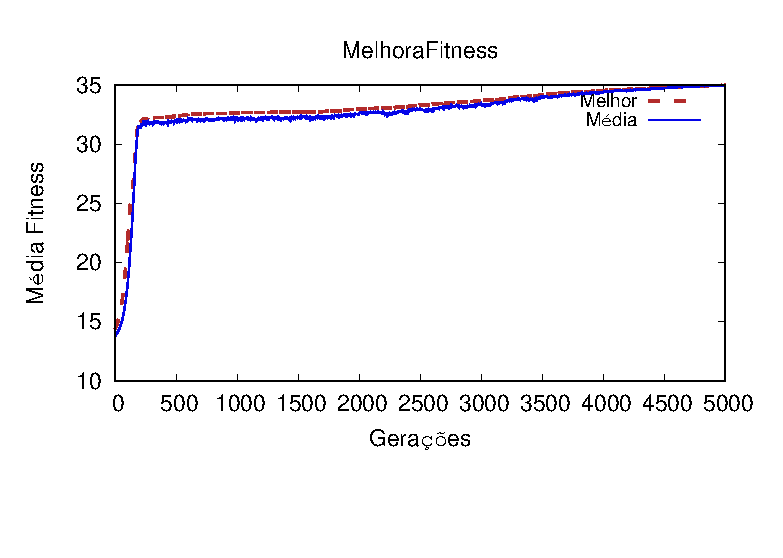
\includegraphics[scale=0.4]{images/p_ackley}} & \raisebox{-.5\height}{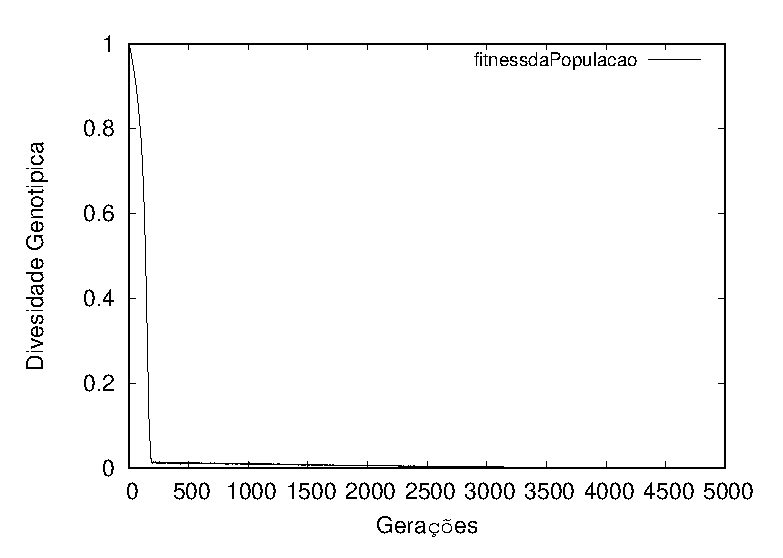
\includegraphics[scale=0.4]{images/d_ackley}} \\ \hline
		Schafel 1,2  & \specialcell{0,01502\\(0,003454)} & \raisebox{-.5\height}{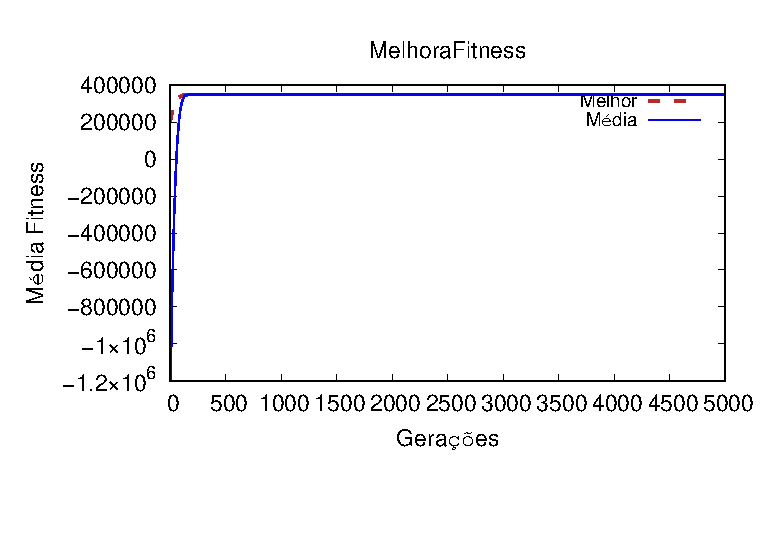
\includegraphics[scale=0.4]{images/p_schaf}} & \raisebox{-.5\height}{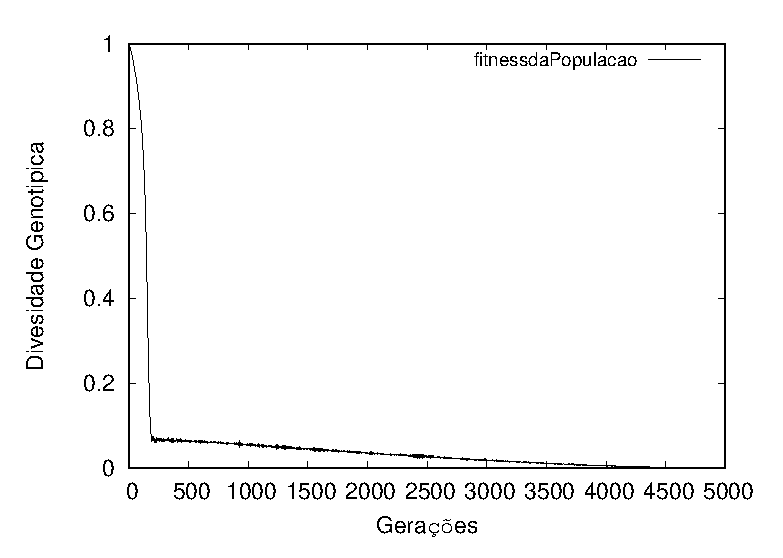
\includegraphics[scale=0.4]{images/d_schaf}} \\ \hline
	\end{tabular}
\end{table}

O resultados atingidos foram muito similares aos resultados obtidos pelo autor \cite{carmelo2008novel} utilizando as mesmas parametrizações, como pode ser visto na Tabela \ref{tb:all_results}. O desvio padrão dos resultados não variarem muito em relação a quantidade de execuções do algoritmo. No artigo foram feitas 30 execuções e neste trabalho foram feitas 10.

\begin{table}[]
\centering
\caption{Comparação dos resultados}\label{tb:all_results}
\begin{tabular}{|c|c|c|c|c|c|}
\hline
\multirow{2}{*}{Funções} & \multicolumn{5}{c|}{Valor de Fitness e desvio padrão}                                                                                                                                                                                                                                                                        \\ \cline{2-6} 
                         & Orig. PSO                                                   & \begin{tabular}[c]{@{}c@{}}Constricted\\ PSO(Gbest)\end{tabular} & \begin{tabular}[c]{@{}c@{}}Constricted\\ PSO(Lbest)\end{tabular} & \begin{tabular}[c]{@{}c@{}}FSS\\ do artigo\end{tabular}   		 & \begin{tabular}[c]{@{}c@{}}FSS desenvolvido\\ pelo autor\end{tabular} \\ \hline
Rosembrock               & \begin{tabular}[c]{@{}c@{}}54.6867\\ (2.8570)\end{tabular}  & \begin{tabular}[c]{@{}c@{}}8.1579\\ (2.7835)\end{tabular}        & \begin{tabular}[c]{@{}c@{}}12.6648\\ (1.2304)\end{tabular}       & \begin{tabular}[c]{@{}c@{}}16.118\\ (0.729)\end{tabular} & \begin{tabular}[c]{@{}c@{}}24,6284\\ (1,68322)\end{tabular}   \\ \hline
Rastrigin                & \begin{tabular}[c]{@{}c@{}}400.7194\\ (4.2981)\end{tabular} & \begin{tabular}[c]{@{}c@{}}140.4876\\ (4.8538)\end{tabular}      & \begin{tabular}[c]{@{}c@{}}144.8155\\ (4.4066)\end{tabular}      & \begin{tabular}[c]{@{}c@{}}13.386\\ (4.005)\end{tabular} & \begin{tabular}[c]{@{}c@{}}13,83\\ (3,70652)\end{tabular}     \\ \hline
Griewank                 & \begin{tabular}[c]{@{}c@{}}1.0111\\ (0.0031)\end{tabular}   & \begin{tabular}[c]{@{}c@{}}0.0308\\ (0.0063)\end{tabular}        & \begin{tabular}[c]{@{}c@{}}0.0009\\ (0.0005)\end{tabular}        & \begin{tabular}[c]{@{}c@{}}0.0027\\ (0.002)\end{tabular} & \begin{tabular}[c]{@{}c@{}}0,008503\\ (0,008108)\end{tabular} \\ \hline
Ackley                   & \begin{tabular}[c]{@{}c@{}}20.2769\\ (0.0082)\end{tabular}  & \begin{tabular}[c]{@{}c@{}}17.6628\\ (1.0232)\end{tabular}       & \begin{tabular}[c]{@{}c@{}}17.5891\\ (1.0264)\end{tabular}       & \begin{tabular}[c]{@{}c@{}}0.0400\\ (0.020)\end{tabular} & \begin{tabular}[c]{@{}c@{}}0,003412\\ (0,000491)\end{tabular} \\ \hline
Schafel                  & \begin{tabular}[c]{@{}c@{}}5.4572\\ (0.1429)\end{tabular}   & \begin{tabular}[c]{@{}c@{}}0.0\\ (0.0)\end{tabular}              & \begin{tabular}[c]{@{}c@{}}0.1259\\ (0.0178)\end{tabular}        & \begin{tabular}[c]{@{}c@{}}0.0808\\ (0.022)\end{tabular} & \begin{tabular}[c]{@{}c@{}}0,01502\\ (0,003454)\end{tabular}  \\ \hline
\end{tabular}
\end{table}

O tempo médio de execução do algoritmo desenvolvido aplicado nos problemas propostos é demostrado na Tabela \ref{tb:time}. os testes foram executados em um Macbook Pro (Retina, Mid 2012), com um processador 2.3 GHz intel \textit{core} i7, 8 GB de memória 1600 MHz DDR3, com o sistema OS X \textit{El Capitan}.

\begin{table}[]
\centering
\caption{Tabela de media de tempo de execução}\label{tb:time}
\begin{tabular}{|c|c|c|c|c|}
\hline
\multicolumn{5}{|c|}{Tempo médio de execução do algoritmo nos problemas em segundos} \\ \hline
Rosembrock       & Rastrigin       & Griewank      & Ackley       & Schafel 1,2      \\ \hline
10,36289         & 10,14934        & 9,48279       & 8,97532      & 9,31242          \\ \hline
\end{tabular}
\end{table}